\documentclass{standalone}
\usepackage{tikz}
\usetikzlibrary{positioning}
\usetikzlibrary{shapes.multipart}
\usetikzlibrary{calc}
\usetikzlibrary{graphs}
\usetikzlibrary{graphs.standard}
\begin{document}
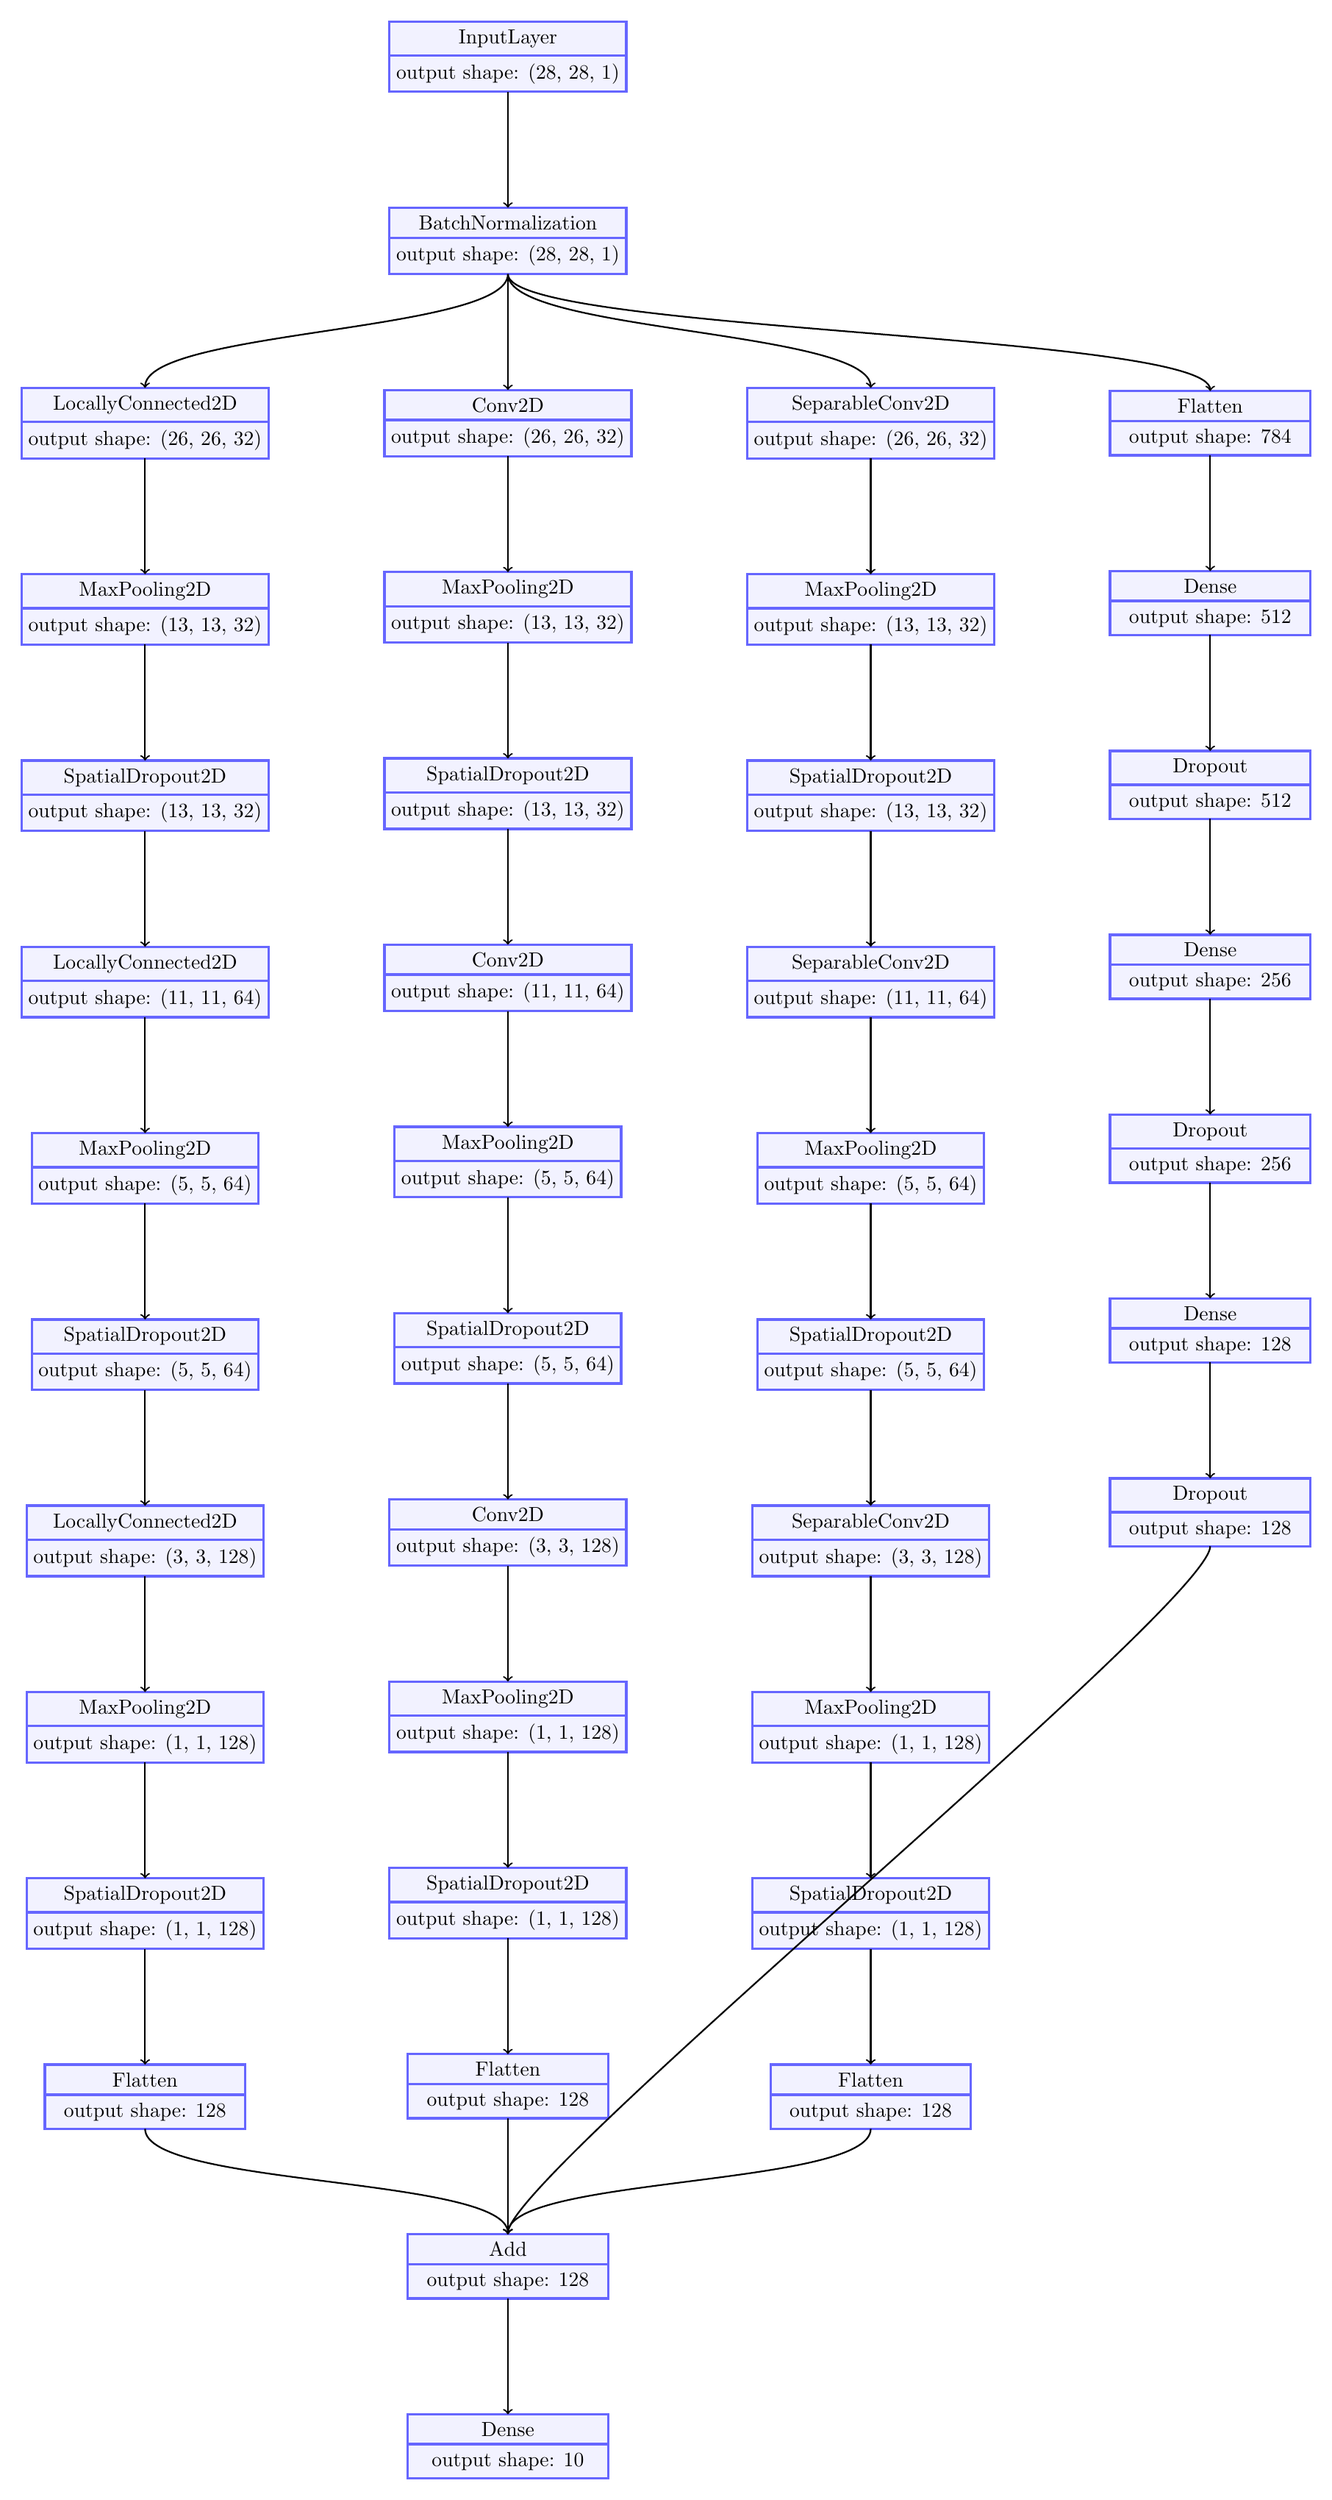
\begin{tikzpicture}
[default_node/.style={rectangle split, rectangle split ignore empty parts, rectangle split parts=2, draw=blue!60, fill=blue!5, very thick, minimum width={width("Batch Normalisation") + 8pt}, node distance=2, outer sep=0pt}, default_path/.style={thick, out=-90, in=90, out distance=1cm, in distance=1cm}]
 \node[default_node] (input_1)  {InputLayer\nodepart{two}output shape: (28, 28, 1)};
\node[default_node] (batch_normalization) [below= of input_1] {BatchNormalization\nodepart{two}output shape: (28, 28, 1)};
\node[default_node] (conv2d) [below= of batch_normalization] {Conv2D\nodepart{two}output shape: (26, 26, 32)};
\node[default_node] (separable_conv2d) [below= of batch_normalization, right= of conv2d] {SeparableConv2D\nodepart{two}output shape: (26, 26, 32)};
\node[default_node] (locally_connected2d) [below= of batch_normalization, left= of conv2d] {LocallyConnected2D\nodepart{two}output shape: (26, 26, 32)};
\node[default_node] (max_pooling2d) [below= of conv2d] {MaxPooling2D\nodepart{two}output shape: (13, 13, 32)};
\node[default_node] (max_pooling2d_3) [below= of separable_conv2d] {MaxPooling2D\nodepart{two}output shape: (13, 13, 32)};
\node[default_node] (max_pooling2d_6) [below= of locally_connected2d] {MaxPooling2D\nodepart{two}output shape: (13, 13, 32)};
\node[default_node] (spatial_dropout2d) [below= of max_pooling2d] {SpatialDropout2D\nodepart{two}output shape: (13, 13, 32)};
\node[default_node] (spatial_dropout2d_3) [below= of max_pooling2d_3] {SpatialDropout2D\nodepart{two}output shape: (13, 13, 32)};
\node[default_node] (spatial_dropout2d_6) [below= of max_pooling2d_6] {SpatialDropout2D\nodepart{two}output shape: (13, 13, 32)};
\node[default_node] (conv2d_1) [below= of spatial_dropout2d] {Conv2D\nodepart{two}output shape: (11, 11, 64)};
\node[default_node] (separable_conv2d_1) [below= of spatial_dropout2d_3] {SeparableConv2D\nodepart{two}output shape: (11, 11, 64)};
\node[default_node] (locally_connected2d_1) [below= of spatial_dropout2d_6] {LocallyConnected2D\nodepart{two}output shape: (11, 11, 64)};
\node[default_node] (flatten_3) [below= of batch_normalization, right= of separable_conv2d] {Flatten\nodepart{two}output shape: 784};
\node[default_node] (max_pooling2d_1) [below= of conv2d_1] {MaxPooling2D\nodepart{two}output shape: (5, 5, 64)};
\node[default_node] (max_pooling2d_4) [below= of separable_conv2d_1] {MaxPooling2D\nodepart{two}output shape: (5, 5, 64)};
\node[default_node] (max_pooling2d_7) [below= of locally_connected2d_1] {MaxPooling2D\nodepart{two}output shape: (5, 5, 64)};
\node[default_node] (dense) [below= of flatten_3] {Dense\nodepart{two}output shape: 512};
\node[default_node] (spatial_dropout2d_1) [below= of max_pooling2d_1] {SpatialDropout2D\nodepart{two}output shape: (5, 5, 64)};
\node[default_node] (spatial_dropout2d_4) [below= of max_pooling2d_4] {SpatialDropout2D\nodepart{two}output shape: (5, 5, 64)};
\node[default_node] (spatial_dropout2d_7) [below= of max_pooling2d_7] {SpatialDropout2D\nodepart{two}output shape: (5, 5, 64)};
\node[default_node] (dropout) [below= of dense] {Dropout\nodepart{two}output shape: 512};
\node[default_node] (conv2d_2) [below= of spatial_dropout2d_1] {Conv2D\nodepart{two}output shape: (3, 3, 128)};
\node[default_node] (separable_conv2d_2) [below= of spatial_dropout2d_4] {SeparableConv2D\nodepart{two}output shape: (3, 3, 128)};
\node[default_node] (locally_connected2d_2) [below= of spatial_dropout2d_7] {LocallyConnected2D\nodepart{two}output shape: (3, 3, 128)};
\node[default_node] (dense_1) [below= of dropout] {Dense\nodepart{two}output shape: 256};
\node[default_node] (max_pooling2d_2) [below= of conv2d_2] {MaxPooling2D\nodepart{two}output shape: (1, 1, 128)};
\node[default_node] (max_pooling2d_5) [below= of separable_conv2d_2] {MaxPooling2D\nodepart{two}output shape: (1, 1, 128)};
\node[default_node] (max_pooling2d_8) [below= of locally_connected2d_2] {MaxPooling2D\nodepart{two}output shape: (1, 1, 128)};
\node[default_node] (dropout_1) [below= of dense_1] {Dropout\nodepart{two}output shape: 256};
\node[default_node] (spatial_dropout2d_2) [below= of max_pooling2d_2] {SpatialDropout2D\nodepart{two}output shape: (1, 1, 128)};
\node[default_node] (spatial_dropout2d_5) [below= of max_pooling2d_5] {SpatialDropout2D\nodepart{two}output shape: (1, 1, 128)};
\node[default_node] (spatial_dropout2d_8) [below= of max_pooling2d_8] {SpatialDropout2D\nodepart{two}output shape: (1, 1, 128)};
\node[default_node] (dense_2) [below= of dropout_1] {Dense\nodepart{two}output shape: 128};
\node[default_node] (flatten) [below= of spatial_dropout2d_2] {Flatten\nodepart{two}output shape: 128};
\node[default_node] (flatten_1) [below= of spatial_dropout2d_5] {Flatten\nodepart{two}output shape: 128};
\node[default_node] (flatten_2) [below= of spatial_dropout2d_8] {Flatten\nodepart{two}output shape: 128};
\node[default_node] (dropout_2) [below= of dense_2] {Dropout\nodepart{two}output shape: 128};
\node[default_node] (add) [below= of flatten] {Add\nodepart{two}output shape: 128};
\node[default_node] (dense_3) [below= of add] {Dense\nodepart{two}output shape: 10};
\draw[->, default_path] (input_1) to (batch_normalization);
\draw[->, default_path] (batch_normalization) to (conv2d);
\draw[->, default_path] (batch_normalization) to (separable_conv2d);
\draw[->, default_path] (batch_normalization) to (locally_connected2d);
\draw[->, default_path] (batch_normalization) to (flatten_3);
\draw[->, default_path] (conv2d) to (max_pooling2d);
\draw[->, default_path] (separable_conv2d) to (max_pooling2d_3);
\draw[->, default_path] (locally_connected2d) to (max_pooling2d_6);
\draw[->, default_path] (max_pooling2d) to (spatial_dropout2d);
\draw[->, default_path] (max_pooling2d_3) to (spatial_dropout2d_3);
\draw[->, default_path] (max_pooling2d_6) to (spatial_dropout2d_6);
\draw[->, default_path] (spatial_dropout2d) to (conv2d_1);
\draw[->, default_path] (spatial_dropout2d_3) to (separable_conv2d_1);
\draw[->, default_path] (spatial_dropout2d_6) to (locally_connected2d_1);
\draw[->, default_path] (conv2d_1) to (max_pooling2d_1);
\draw[->, default_path] (separable_conv2d_1) to (max_pooling2d_4);
\draw[->, default_path] (locally_connected2d_1) to (max_pooling2d_7);
\draw[->, default_path] (flatten_3) to (dense);
\draw[->, default_path] (max_pooling2d_1) to (spatial_dropout2d_1);
\draw[->, default_path] (max_pooling2d_4) to (spatial_dropout2d_4);
\draw[->, default_path] (max_pooling2d_7) to (spatial_dropout2d_7);
\draw[->, default_path] (dense) to (dropout);
\draw[->, default_path] (spatial_dropout2d_1) to (conv2d_2);
\draw[->, default_path] (spatial_dropout2d_4) to (separable_conv2d_2);
\draw[->, default_path] (spatial_dropout2d_7) to (locally_connected2d_2);
\draw[->, default_path] (dropout) to (dense_1);
\draw[->, default_path] (conv2d_2) to (max_pooling2d_2);
\draw[->, default_path] (separable_conv2d_2) to (max_pooling2d_5);
\draw[->, default_path] (locally_connected2d_2) to (max_pooling2d_8);
\draw[->, default_path] (dense_1) to (dropout_1);
\draw[->, default_path] (max_pooling2d_2) to (spatial_dropout2d_2);
\draw[->, default_path] (max_pooling2d_5) to (spatial_dropout2d_5);
\draw[->, default_path] (max_pooling2d_8) to (spatial_dropout2d_8);
\draw[->, default_path] (dropout_1) to (dense_2);
\draw[->, default_path] (spatial_dropout2d_2) to (flatten);
\draw[->, default_path] (spatial_dropout2d_5) to (flatten_1);
\draw[->, default_path] (spatial_dropout2d_8) to (flatten_2);
\draw[->, default_path] (dense_2) to (dropout_2);
\draw[->, default_path] (flatten) to (add);
\draw[->, default_path] (flatten_1) to (add);
\draw[->, default_path] (flatten_2) to (add);
\draw[->, default_path] (dropout_2) to (add);
\draw[->, default_path] (add) to (dense_3);
\end{tikzpicture}\end{document}